\documentclass{article}
\usepackage{amsmath}
\usepackage{graphicx}
\usepackage{longtable}
\usepackage{makecell}
\usepackage[most]{tcolorbox}
\usepackage{listings}

\title{DRLND Navigation-Report}
\date{2018-11-10}
\author{Matthias Schinacher matthias.schinacher@googlemail.com}

\begin{document}

\maketitle
\tableofcontents
\newpage

\section{Intro}
The project is a homework assignment for Udacity's \textbf{Deep Reinforcement Learning Nano Degree}.
The project ist the first one called \textit{Navigation}.
\\
The project environment is a course provided version of the Unity "Banana Collector"
environment of the ML- agents Unity has on the respective github- page.
The environment has an "agent" with 4 possible actions and is full of bananas
that want to be collected if yellow (increases score) and avoided if purple
(decreases score if hit by one). The task is to achieve a score of at least 13
per episode with a deep reinforcement algorithm.
\\
For this project I chose to implement Q- learning with experience replay and
optional priority replay in a python script to be invoked from command line.
\\
The model for the Q- function is a simple neural network with 3 layers,
where the first 2 layers are simple linear layers followed by a ReLU activation
and the last layer is a linear layer \textbf{without} an activation function.
This model maps the \textit{state} directly to the state-action function Q
(or rather an approximation of Q); the output of the final layer is interpreted
as the approximations for the 4 possible \textit{actions}.
\\
Thus this model has 2 size parameters, as the input-size is given by the state size (37)
and the output size is given by the number of available actions (4).

\section{Implementation}
\subsection{python script}
The script is named $ms\_drlndnav\_pr.py$ and must be invoked from the command
line with exactly one parameter, the name of the ".ini"- file (a.k.a. command file),
that has all the parameters.

\paragraph{Parameters}
The parameters listed in the command file come in various sections. The basic format
is similar to the Windows style INI files and is the one that pythons $configparser$
module uses (as the module is used in the script).

\subparagraph{Example}
:\\
\tiny
\texttt{
{[global]} \\
runlog = test6.log \\
{[mode]} \\
train = 1 \\
{[rand]} \\
seed = 4719 \\
{[model]} \\
h1 = 17 \\
h2 = 11 \\
save\_file = test6.model \\
save\_best\_file = test6.best.model \\
save\_transitions\_file = test6.transitions \\
{[hyperparameters]} \\
episodes           = 1000 \\
warmup\_episodes    = 10 \\
epsilon\_episodes   = 200 \\
epsilon\_start      = 0.99 \\
epsilon\_end        = 0.01 \\
replay\_buffersize  = 30000 \\
replay\_batchsize   = 300 \\
replay\_steps       = 1 \\
prio\_replay        = False \\
q\_reset\_steps      = 30 \\
gamma              = 0.99 \\
learning\_rate      = 0.001
}

\normalsize

\subparagraph{Description}
:\\
\begin{tabular}{ |l|r|l|c| }
  \hline
  \multicolumn{4}{|c|}{Parameters} \\
  \hline
Section & Name & Description & Default \\
  \hline
\multicolumn{4}{|l|}{\textbf{global}} \\
               & runlog & name of the logfile to use & \texttt{run.log} \\
\multicolumn{4}{|l|}{\textbf{mode}} \\
               & train & whether we're in training mode & \texttt{True} \\
               & show & \makecell[tl]{flag, whether to show \\ the game in "human time"} & \texttt{False} \\
\multicolumn{4}{|l|}{\textbf{rand}} \\
               & seed & \makecell[tl]{seed for \\ random number generation} & \makecell[tc]{no explicit \\ random seeding performed} \\
\multicolumn{4}{|l|}{\textbf{model}} \\
               & h1 & \makecell[tl]{first size- parameter \\ for the NN- model} & \texttt{10} \\
               & h2 & \makecell[tl]{second size- parameter \\ for the NN- model} & \texttt{10} \\
               & load\_file & \makecell[tl]{load model from this file} & \makecell[tc]{"\texttt{Q.model}" \\ if not in training mode} \\
               & load\_transitions\_file & \makecell[tl]{load replay-memory transitions \\ from this file} & \texttt{None} \\
               & save\_file & \makecell[tl]{save final Q- model \\ to this file} & \makecell[tc]{"\texttt{Q.out.model}" \\ if in training mode} \\
               & save\_best\_file & \makecell[tl]{save Q- model from episode \\ with highest score to this file} & \makecell[tc]{\texttt{None} \\ if in training mode} \\
               & save\_transitions\_file & \makecell[tl]{save replay-memory transitions \\ to this file} & \texttt{None} \\
\multicolumn{4}{|l|}{\textbf{hyperparameters}} \\
               & episodes & number of episodes to run & \texttt{1000} \\
               & warmup\_episodes & \makecell[tl]{epiosodes to run with \\ pure random sampling} & \texttt{10} \\
               & epsilon\_episodes & \makecell[tl]{number of episodes over \\ which to descrease $\epsilon$} & \texttt{100} \\
               & epsilon\_start & start- value for $\epsilon$ & \texttt{1.0} \\
               & epsilon\_end & final value for $\epsilon$ & \texttt{0.01} \\
               & replay\_buffersize & size of the replay memory & \texttt{50000} \\
               & replay\_batchsize & \makecell[tl]{number of transitions to sample \\ per optimizing step} & \texttt{300} \\
               & replay\_steps & \makecell[tl]{game-steps between \\ each optimizing step} & \texttt{1} \\
               & prio\_replay & \makecell[tl]{flag, whether to use \\ priority replay} & \texttt{False} \\
               & q\_reset\_steps & \makecell[tl]{reset the parameters \\ of the "fixed" Q- model \\ after this many steps} & \texttt{50} \\
               & gamma & $\gamma$ & \texttt{0.99} \\
               & learning\_rate & the learning rate & \texttt{0.001} \\
%               &  &  & \texttt{} \\
\hline
\end{tabular}
\textbf{Note:} the $show$- parameter determines, if the unity engine should
show the episodes slower, as to allow a human observer to follow the game; therefor
it determines the value given to the unity- environment as the parameter $train\_mode$.
\\
The $train$- parameter of the script determines, if the algorithm will be learning
from new transitions.

\subsection{Using the script/ Implementation}
\paragraph{Dependencies}
The script has runtime dependencies; these are the ones as described in the
project instructions; I will therefore refrain from detailing the dependencies \textit{here}.

\paragraph{Details/ algorithm}
The script is invoked from the command line as a python script with one parameter,
a file-name from which to read all the parameters governing the algorithm.
\\
Example:\\
\texttt{python ms\_drlndnav\_pr.py test6.ini}
\\
The algorithm implemented is basically Q- learning with the optimizing step
using a replay-memory buffer from which the transitions to be used are sampled.
The neural network approximizing the Q- state-action function is implemented
using \texttt{pytorch} and the optimizer used is "Adam" from said package.
\\
The replay memory-buffer is implemented as a simple list with a specified capacity (\textit{replay\_buffersize}),
where the oldest entry is overwritten by the newest entry, if the capacity is already
fully used.
\\
The script uses a specified number (\textit{replay\_batchsize}) of transitions
to perform the optimization step; by default this optimization step is performed
for every game step, but this can be changed via \textit{replay\_steps}.
\\
Optionally the script implements a crude form of priority replay (parameter \textit{prio\_replay}).

\subparagraph{Loading and saving models/ pretraining}
The script is able to save the model- state of the neural network as well as
the transitions in the replay-memory to file and/or load these from file
at the beginning of a script-run.
\\
This enables us to use the results of a previous training as the pretraining
for further model-training runs with changed parameters, as long as the model-
size parameters are not changed (\textit{h1} and \textit{h2}).
\\
\textbf{Note:} the saving/loading of the models is achieved using the methods
$torch.load(..)$ and $torch.save(..)$ which are \textbf{not} easily human readable.\\
The loading/saving of the transitions (the replay buffer) is done via
the standard python module $pickle$, which also uses a binary format. 

\subparagraph{Non training mode}
If the \textit{train}- parameter is set to $False$, the script performs
a scenario - plays the game - without any update to the neural network,
not learning anything. If used, one must also set a model- file to be loaded!
\\
Whether the unity framework will show the game episodes in a speed, that allows
a human observer to follow the game, can be set with parameter \textit{show}.
As the program needs to know with what probability $\epsilon$ to sample randomly
instead of greedy using the Q- value approximation of the model, at least
the parameter \textit{epsilon\_end} should be set (but one can also use the
others).

\subparagraph{Log- output}
Each script- execution/ training-run a log-file (with configurable name) is
written; this file has informational text- output - including the parameters used -
and uses the '\#' character in the first column, so certain programs/ tools will
know to ignore these \textit{commen-style} outputs.
\\
The main output in the logfile is a (non '\#'-) textline per episode containing
the episode, the score the episode reached, the average score of the last 100
episodes (or 0, if it's an episode before the 100th), the number of steps executed
(which seem to be always 300?) and the epsilon- value used for this episode
separated by a blank.
The logfile can thus be read by certain programs/ tools as some sort
of time-series for the score and the average-100-last-episodes-score; one such
tool is \textbf{gnuplot}, with which I created the graphics contained in the report.

\section{Results} \label{res}
\subsection{What I did}
I used my program/ script mainly to try out different sets of the size parameters
\textit{h1} and \textit{h2} to find some settings, that would satisfy the
\textit{"at least score 13"}- requirement. Once I had found a combination of these
that would yield a long enough run \textit{above score 13} (command- file $test4.ini$),
I experimented mainly with minor modifications of these.

\subsection{Basic results}
As can seen in the graph-plots, the algorithm with the resulting model(s)
is not able to run the game/ simulation above a score of 13 for subsequent episodes
over a prolonged time. The resulting score per episode fluctuates quite subtantially.
\\
\textbf{However} what the algorithm/ model \textbf{is able} to deliver is quite a
large run of episodes for which the "average over the last 100 scores" is solid
above 13 (see results for $test4.ini$ or $test4c.ini$).

\paragraph{Command files/ INI- files}
Each command file (a.k.a. INI- file) represents one \textit{experiment} (program/ script- run).
See the list below for an overview of these experiments/ command files
(refer to the actual files for details of all hyperparameters).
\\

\begin{tabular}{ |l|l| }
  \hline
Filename & Description \\
  \hline
$test4.ini$ & \makecell[tl]{first successful experiment reaching "score 13", \\ with size- parameters $h1$ and $h2$ each 10 \\ (no priority-replay!)} \\
$test4c.ini$ & \makecell[tl]{mostly like $test4.ini$, uses model \\ from latter as pre-training} \\
$test4c2.ini$ & \makecell[tl]{like $test4.ini$, basically a continuation of it \\ (with model loaded as pre-training); \\ but different $\epsilon$} \\
$test4c3.ini$ & \makecell[tl]{same as $test4c2.ini$ \\ but changes \textit{replay\_steps}} \\
$test4c4.ini$ & \makecell[tl]{same as $test4c.ini$ \\ but with priority-replay} \\
$test4c5.ini$ & \makecell[tl]{size- parameters $h1$ and $h2$ are 8 and 6} \\
$test4c6.ini$ & \makecell[tl]{size- parameters $h1$ and $h2$ are 17 and 11} \\
  \hline
\end{tabular}

\paragraph{Graph- plots}

\textit{(All plots are score per episode plus average score of the last 100 episodes per episode)}
\\
\begin{tabular}{ |c|c| }
  \hline
  \texttt{test4.ini} & \texttt{test4c.ini} \\
  \hline
  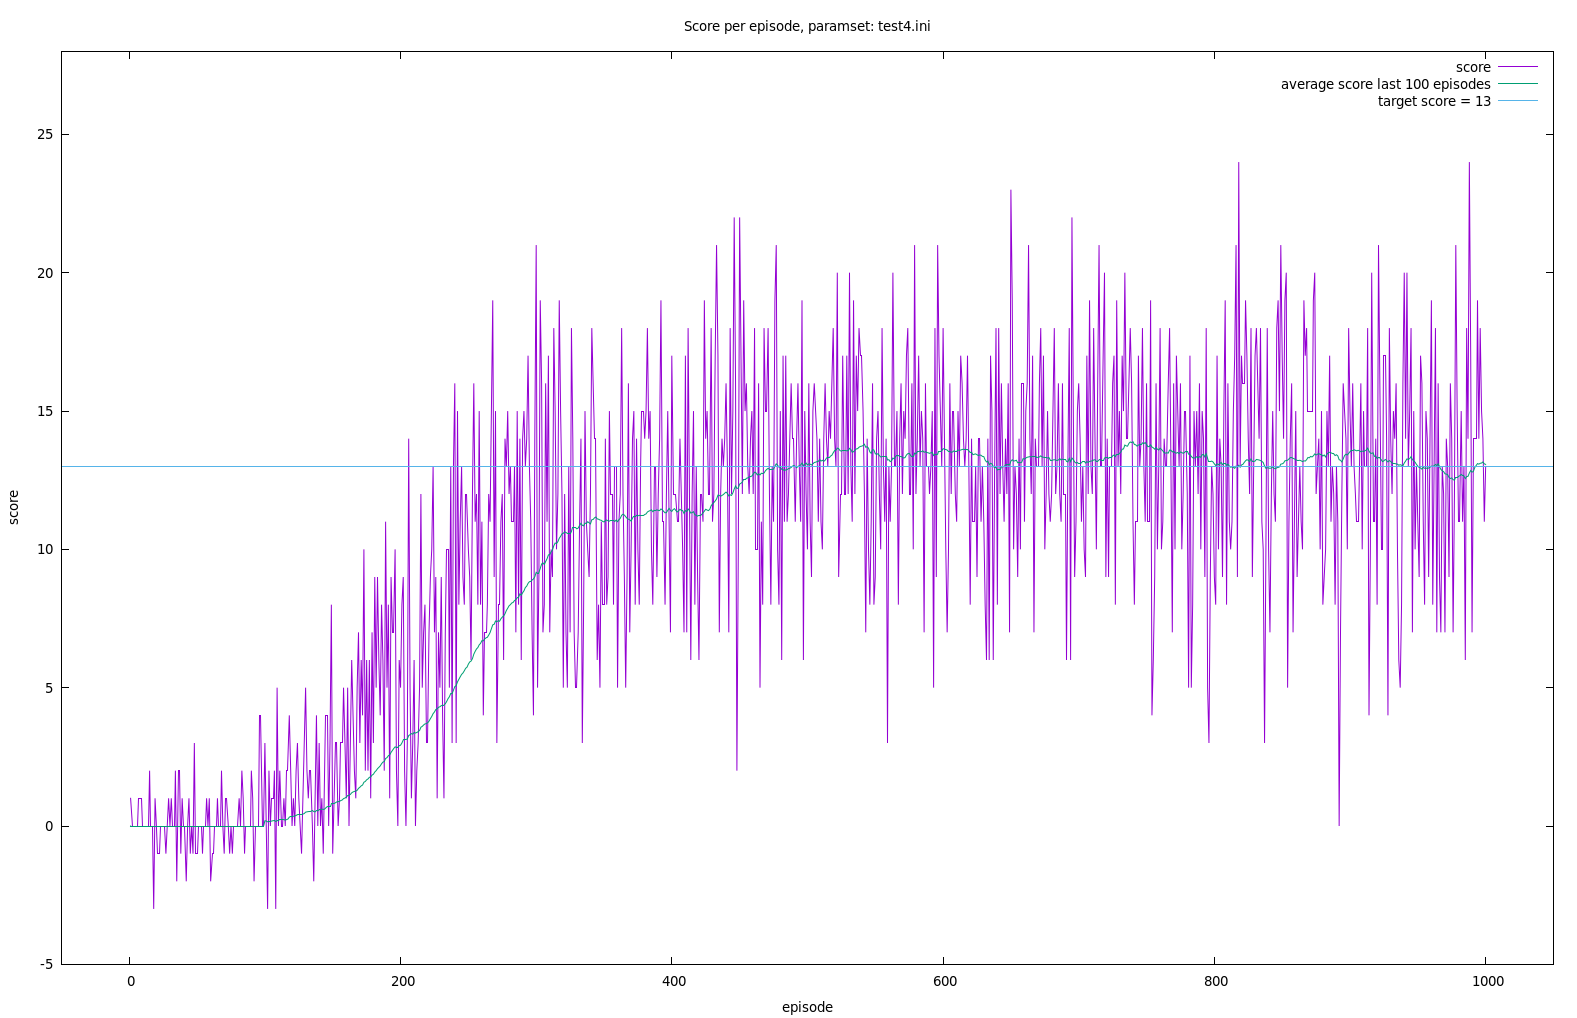
\includegraphics[scale=0.12]{test4.png} & \includegraphics[scale=0.12]{test4c.png} \\
  \hline
  \texttt{test4c2.ini} & \texttt{test4c3.ini} \\
  \hline
  \includegraphics[scale=0.12]{test4c2.png} & \includegraphics[scale=0.12]{test4c3.png} \\
  \hline
  \texttt{test4c4.ini} &  \\
  \hline
  \includegraphics[scale=0.12]{test4c4.png} &  \\
  \hline
  \texttt{test5.ini} & \texttt{test6.ini} \\
  \hline
  \includegraphics[scale=0.12]{test5.png} & \includegraphics[scale=0.12]{test6.png} \\
  \hline
\end{tabular}

\subsection{Remarks/ discussion}
The actual goal/ target I treid to reach was a prolonged run of episodes
for which the average score of "the last 100 episodes" is at least 13.
\\
$test4.ini$ achieves that goal and the algorithm "learns" the neccessary model
within 476 episodes. The \textit{smaller} $test5.ini$- model seems to allow
to reach that goal by 446 episodes - thus learns faster - but seems not be be
able to "hold onto" the 13, is kind of unstable.\\
The \textit{bigger} model of $test5.ini$ seems to be more stable (regarding the
"last 100 episodes"- metric, but also slower and reaches the 13 by 611 episodes.\\
As already mentioned, all runs/ experiments fail to learn a model that guarantees
a score of 13 for a sequence of episode, all fluctuate substanially per episode.
\\
The experiment with priority-replay ($test4c4.ini$) suggests, that either priority-replay
is not beneficial for the game-scenario, or maybe the implementation suffers from a bug,
or maybe the missing modification of the update rule (not implemented) is a must.

\subsection{Some more results}

\begin{tabular}{ |l|l| }
  \hline
Filename & Description \\
  \hline
$test4X.ini$ & \makecell[tl]{mostly like $test4.ini$, uses model \\ from latter as pre-training} \\
$test4X2.ini$ & \makecell[tl]{loads model from $test4.ini$, \\ training mode if off!} \\
  \hline
\end{tabular}

The interesting one of these is the experiment of $test4X2.ini$, since it uses
a pre-trained model \textbf{without} further training the model. As can be seen,
the model used allows largely for our goal of "average score of the last 100
episodes at least 13", but still fluctuates bigly per episode.

\begin{tabular}{ |c| }
  \hline
  \texttt{test4X.ini}  \\
  \hline
  \includegraphics[scale=0.2]{test4X.png} \\
  \hline
  \texttt{test4X2.ini}  \\
  \hline
  \includegraphics[scale=0.2]{test4X2.png} \\
  \hline
\end{tabular}

\section{Possible improvements}
\subsection{Algorithm}
\paragraph{Random sampling}
The algorithm chooses a random sample among the 4 possible actions with
the probability of $\epsilon$ (which is usually quite small); but in the event
of this random sampling, the probability of each of the 4 actions is the same.
\\
A possible improvement could be to choose between the 4 actions in some manner
dependent on the Q- value for the actions, prefering the ones with a higher value.
This in combination with a higher value of epsilon might be beneficial in situations,
where for example 2 actions have almost the same "current" Q- value approximation
while the other 2 actions have a much lower value. Of the 2 "top" actions only
one is chosen with pobability $1 - \epsilon$, even though maybe the other one should
sampled almost as often.

\paragraph{Priority replay}
The algorithm/ the script \textit{does} impelement priority replay (as an option), but only
with the raw $\delta$- values. This does not seem to improve the algorithm; it might
be good to try the modification to the update rule (sampling weights) and/or the
additional hyper parameter $a$, that controls the degree of uniform sampling.

\paragraph{Tweaking $\epsilon$- decay}
The $\epsilon$- decay I used was rather simple, a start value, an end value and
a number of episodes in which to decrease the value bewteen these linearily.
\\
It would be interesting to see, if another form of $\epsilon$ decay (non linear)
would have any impact.

\subsection{NN- Model}
The model for the neural network I used was very simple. My gut feeling is,
that a much deeper network or bigger layers would not be very promising,
but one could try.
\\
What I \textbf{really} would like to try in the future however is using different
types of layers. Maybe convolutional layers instead of the linear ones and
activation functions other then ReLU (maybe $tanh$ activations).
The Q- function approximation with my "linear and ReLU"- model seems to give rise
to an erratic behaviour of the agent (this is my impression, when watching in
$show$- mode with the model), maybe these other layers/activations might smooth
the agent.

\section{Result model}
As described in the section \ref{res} the model for experiment $test4.ini$ is
my result model; as the script saved actually 2 models, the final one and the
one at the end of the episode with the highest score, I choose the latter
($test4.best.model$) a \textit{result model for the task/ project}.
\\
To recap, my neural network (using pytorch) has 3 linear layers with 2 ReLU
activations between them.\\
\\
\tiny
\begin{tabular}{ |l|r|r|r|r|r|r|r|r|r|r| }
  \hline
\multicolumn{11}{|l|}{\textbf{Weights: first linear layer (10x37)}} \\
  \hline
Row/Col & 1,11,.. & 2,12,.. & 3,12,.. & 4,.. & 5,.. & 6,.. & 7,.. & 8,..& 9,..& 10,.. \\
  \hline
1 & 0.7284 & 0.4451 & 0.5770 & 0.6038 & 0.0178 & 0.5494 & 0.7112 & 0.7281 & 0.7345 & 0.1827 \\
  & 0.2747 & 0.2970 & 0.2803 & 0.2258 & 0.0198 & 0.4788 & 0.2270 & 0.2586 & 0.2617 & 0.0137 \\
  & 0.4665 & 0.5984 & 0.5894 & 0.4759 & 0.0861 & 0.3718 & 0.5941 & 0.4081 & 0.4736 &-0.0720 \\
  & 0.4760 & 0.1903 & 0.2055 & 0.5565 & 0.6621 & -0.0527 & 0.0353 & & & \\
2 & -0.1642 & 0.1435 & 0.1091 & 0.1639 & 0.1639 & 1.3126 & -1.9600 & -1.9593 &-1.8851 &-4.8989 \\
  & 0.0431 & 0.1173 & 0.0515 & 0.1304 & 0.1497 & 0.0524 & 0.2186 & 0.1833 & 0.1522 & 0.1481 \\
  & 0.1206 & 0.2612 & 0.1785 & 0.4554 & 0.0200 & 0.0942 & 0.2407 & 0.4419 & 0.2407 &-0.0851 \\
  & 0.2434 & 0.4942 & 0.5666 & 0.8525 & 0.5180 & 0.0604 & 0.0107 & & & \\
3 & 0.4575 & 0.4587 & 0.4418 & 0.4428 &-0.2156 & 0.4017 & 0.4019 & 0.1642 & 0.2583 & 0.0835 \\
  & 0.3032 & 0.2742 & 0.3057 & 0.0292 &-0.5276 & 0.0651 & 0.1777 &-0.0148 & 0.0384 &-0.6452 \\
  &-0.2594 & 0.1701 &-0.2055 & 0.0068 &-0.2395 & 0.3919 & 0.2091 & 0.2338 & 0.0605 &-0.0193 \\
  &-1.1103 & 0.9839 & 1.2349 &-0.2261 &-3.2658 &-0.0182 &-0.0059 & & & \\
4 & 0.1282 & 0.1771 & 0.0908 & 0.1449 &-0.0103 & 0.2509 & 0.1184 &-0.0462 & 0.1747 &-0.0154 \\
  & 0.2375 & 0.2700 & 0.3128 & 0.2220 & 0.0173 & 0.1006 & 0.0488 & 0.1383 & 0.3490 & 0.2106 \\
  & 0.1793 & 0.1890 & 0.2415 & 0.2761 & 0.0228 & 0.7293 &-0.1479 & 0.0892 & 0.8269 & 1.3420 \\
  & 0.4237 & 0.6185 & 0.2465 &-0.9567 &-2.5973 & 0.0198 &-0.0067 & & & \\
5 & 0.6973 & 0.5472 & 0.6367 & 0.6043 & 0.0159 & 0.3936 & 0.3432 & 0.6624 & 0.2514 &-0.2076 \\
  & 0.2073 & 0.2428 & 0.1707 & 0.3936 & 0.0866 & 0.3564 & 0.1099 & 0.1618 &-0.1041 &-0.4952 \\
  & 0.3736 & 0.3725 & 0.2738 & 0.1957 & 0.0127 &-0.1175 & 0.7720 & 0.3778 &-0.2382 &-1.3762 \\
  & 0.5207 & 0.6262 & 0.1242 & 0.1927 &-1.6857 &-0.0300 & 0.0115 & & & \\
6 & 0.0253 &-0.1518 &-0.0079 & 0.0502 & 0.1365 &-0.2260 &-0.1039 & 0.1791 & 0.0298 & 0.2347 \\
  & 0.0471 & 0.0768 & 0.1856 & 0.1528 & 0.0844 &-0.0918 &-0.0885 &-0.0517 &-0.0064 & 0.3238 \\
  & 0.9025 &-1.4990 &-1.3724 &-0.9512 &-4.9401 &-0.0835 & 0.2286 & 0.2001 & 0.2367 &-0.0457 \\
  & 0.2723 & 0.3861 & 0.3749 & 0.4747 & 0.2489 & 0.1388 & 0.0536 & & & \\
7 & 0.1487 & 0.2293 & 0.4352 & 0.2539 &-0.0188 & 0.3637 & 0.2053 &-0.0056 & 0.2037 &-0.0222 \\
  & 0.4198 & 0.5404 & 0.3993 & 0.1536 &-0.3698 &-0.1687 & 0.2762 & 0.1069 & 0.4962 & 0.6675 \\
  & 0.1251 & 0.3229 & 0.3999 & 0.4688 &-0.0552 &-0.2042 & 0.6131 & 0.7273 &-0.1236 &-0.8534 \\
  & 0.4894 & 0.3267 & 0.2585 &-0.2687 &-0.6904 & 0.0127 & 0.0686 & & & \\
8 & 0.3154 & 0.2913 & 0.3331 & 0.1735 &-0.0971 &-0.0285 & 0.0655 & 0.1385 & 0.1707 &-0.0382 \\
  & 0.2372 &-0.2379 &-0.2240 &-0.1344 &-0.5503 &-0.1582 & 0.5722 & 0.2566 &-0.0058 &-0.5098 \\
  & 0.1663 & 0.2884 &-0.0933 &-0.1977 &-0.4197 & 0.6533 & 0.0810 & 0.0929 & 0.6966 & 0.8923 \\
  &-0.2537 &-0.1914 & 0.1261 & 0.8796 & 1.1088 & 0.0858 & 0.0071 & & & \\
9 & 0.2996 & 0.1677 & 0.4225 & 0.4432 & 0.2843 & 0.3976 & 0.2358 & 0.2723 & 0.1536 &-0.1615 \\
  & 0.0945 & 0.1099 & 0.0943 & 0.1373 & 0.0932 &-0.2333 & 0.9769 & 0.6094 & 0.5311 & 2.0743 \\
  & 0.3969 & 0.2826 & 0.3545 & 0.1719 &-0.1371 &-4.2956 & 1.1820 & 0.8422 &-0.6651 &-2.4409 \\
  & 0.1368 & 0.1347 & 0.2328 & 0.0418 & 0.0542 &-0.0326 &-0.0032 & & & \\
10& 0.6296 & 0.6470 & 0.5274 & 0.6949 & 0.0505 & 0.3634 & 0.3725 &-0.0427 & 0.1691 &-0.2843 \\
  & 0.7060 & 0.5514 & 0.5985 & 0.5779 &-0.0128 & 0.2214 & 0.4288 & 0.3920 & 0.3203 &-0.1728 \\
  & 0.8080 & 0.5878 & 0.5746 & 0.5311 &-0.2822 &-0.1809 & 1.0708 & 0.9328 &-0.4926 &-1.9445 \\
  & 0.3858 & 0.7469 & 0.9445 & 0.0555 &-0.4865 & 0.0351 &-0.0384 & & & \\
  \hline
\multicolumn{11}{|l|}{\textbf{Bias: first linear layer (10)}} \\
  \hline
 & 0.2428 & -0.0704 & -0.1345 & 0.1645 & -0.0810 & -0.4909 & -0.4218 & -0.5246 & -0.2332 & 0.3380 \\
  \hline
\multicolumn{11}{|l|}{\textbf{Weights: second linear layer (10x10)}} \\
  \hline
Row/Col & 1 & 2 & 3 & 4 & 5 & 6 & 7 & 8 & 9 & 10 \\
  \hline
 1 & 0.1709 & 1.0977 & 0.7487 &-0.6399 & 0.0749 &-0.6871 &-0.4686 &0.2392 & 0.2629 &-0.4470 \\
 2 & -0.0132 & 0.4071 & 0.0331 &-0.3639 & 0.0529 &-0.0990 & 0.3005 &-0.0449 &-0.2492 & 0.2732 \\
 3 & -0.1888 & 0.7423 &-0.5210 & 0.0828 &-0.1780 &-0.4697 &-0.2159 &0.1838 & 0.5265 &-0.1205 \\
 4 &  0.5250 &-0.0168 & 0.0375 &-0.3340 & 0.3123 & 0.0547 & 0.4268 &-0.0515 &-0.8815 & 0.3730 \\
 5 &  0.0394 &-0.4144 & 0.0395 &-0.2337 & 0.2819 & 1.0401 &-0.3293 &-0.1860 &-0.8132 & 0.4819 \\
 6 & -0.0766 & 0.2056 &-0.0018 & 0.5585 &-0.2392 & 0.5279 &-0.3815 &0.3447 & 0.9636 &-0.4448 \\
 7 & -0.3756 &-0.3144 &-1.8101 & 0.6762 & 0.5495 &-0.4956 & 0.1216 &-0.1097 & 0.1037 &-0.1714 \\
 8 &  0.0713 &-0.2342 & 0.1115 &-0.3384 & 0.0521 & 0.7158 & 0.1937 &-0.2173 & 0.0101 &-0.3810 \\
 9 & -0.2325 & 0.1013 &-0.2682 & 0.4572 &-0.0457 & 0.5359 & 0.0884 &0.5409 & 0.3778 &-0.0567 \\
10 &  0.4017 & 0.0866 &-0.4242 & 0.4539 & 0.0298 & 0.0421 &-0.0724 &-0.1260 &-0.1497 & 0.3004 \\ 
  \hline
\multicolumn{11}{|l|}{\textbf{Bias: second linear layer (10)}} \\
  \hline
 & 0.7262 & 1.0303 & -0.4341 & 1.0356 & 0.5020 & 0.5283 & 0.0408 & 0.7571 & 0.7692 & 0.9097 \\
  \hline
\multicolumn{11}{|l|}{\textbf{Weights: third linear layer (4x10)}} \\
  \hline
Row/Col & 1 & 2 & 3 & 4 & 5 & 6 & 7 & 8 & 9 & 10 \\
  \hline
1 & 0.1743 & 0.3245 &-0.0795 & 0.3006 & 0.1421 & 0.4010 & 0.6122 &0.0588 & 0.0727 &0.4349 \\
2 & 0.1686 & 0.2431 &-0.0423 & 0.2576 & 0.1847 & 0.3751 & 0.5488 &-0.1453 & 0.0439 & 0.4147 \\
3 & 0.0643 & 0.2912 &-0.2521 & 0.4252 & 0.1450 & 0.3833 & 0.6694 &0.1801 & 0.2982 & 0.1768 \\
4 &-0.0629 & 0.3338 &-0.2007 & 0.6259 & 0.1865 & 0.8772 & 0.4972 &-0.2213 &-0.2589 & 0.1077 \\
  \hline
\multicolumn{11}{|l|}{\textbf{Bias: third linear layer (4)}} \\
  \hline
& 0.7185 & 0.8497 & 0.8610 & 0.7685 & & & & & & \\
  \hline
  
\end{tabular}

\end{document}
